\documentclass[10pt,twocolumn,a4paper]{article}
% High-quality conference proceedings styling with enhanced typography
\usepackage[utf8]{inputenc}
\usepackage[T1]{fontenc}
\usepackage[margin=0.75in,columnsep=0.25in]{geometry}
\usepackage{lmodern}
\usepackage[protrusion=true,expansion=false]{microtype}
\usepackage{graphicx}
\usepackage{booktabs}
\usepackage{amsmath,amssymb,mathtools}
\usepackage{authblk}
\usepackage{enumitem}
\usepackage{url}
\usepackage{xcolor}
\usepackage{titlesec}
\usepackage{balance}
\usepackage[font=small,labelfont={bf,color=navyblue},skip=4.5pt]{caption}
\usepackage{hyperref}
\usepackage[capitalize,noabbrev]{cleveref}

% Professional academic color palette
\definecolor{navyblue}{RGB}{12, 45, 110}
\definecolor{charcoal}{RGB}{35, 35, 35}

\hypersetup{
    colorlinks=true,
    linkcolor=navyblue,
    citecolor=navyblue,
    urlcolor=navyblue
}

% Spacing & Layout
\setlength{\parindent}{1.1em}
\setlength{\parskip}{0pt}
\setlength{\affilsep}{0.45em}
\renewcommand\Authfont{\large\bfseries}
\renewcommand\Affilfont{\small\normalfont}
\renewcommand\Authands{, and }
\setlist[enumerate]{leftmargin=*,itemsep=1.2pt,topsep=2.5pt,parsep=0pt}
\setlist[itemize]{leftmargin=*,itemsep=1.2pt,topsep=2.5pt,parsep=0pt}
\setlength{\textfloatsep}{5pt plus 2pt minus 2pt}
\setlength{\floatsep}{4pt plus 2pt minus 2pt}
\setlength{\intextsep}{4pt plus 2pt minus 2pt}
\setlength{\dbltextfloatsep}{5pt plus 2pt minus 2pt}
\setlength{\dblfloatsep}{4pt plus 2pt minus 2pt}
\setcounter{topnumber}{3}
\setcounter{dbltopnumber}{3}
\renewcommand{\topfraction}{0.95}
\renewcommand{\dbltopfraction}{0.95}
\renewcommand{\textfraction}{0.05}
\renewcommand{\floatpagefraction}{0.85}
\renewcommand{\dblfloatpagefraction}{0.85}
\emergencystretch=2.5em
\clubpenalty=10000
\widowpenalty=10000

% Section Heading Formatting (Bold, Larger, Styled with Deep Navy)
\renewcommand{\thesection}{\Roman{section}}
\renewcommand{\thesubsection}{\thesection.\arabic{subsection}}

\titleformat{\section}
  {\large\bfseries\color{navyblue}}
  {\thesection.}{0.6em}{\MakeUppercase}
\titlespacing*{\section}{0pt}{8.5pt plus 2pt minus 1pt}{3.5pt plus 1pt minus 1pt}

\titleformat{\subsection}
  {\normalsize\bfseries\color{charcoal}}
  {\thesubsection}{0.5em}{}
\titlespacing*{\subsection}{0pt}{6.5pt plus 2pt minus 1pt}{2.5pt plus 1pt minus 1pt}

\titleformat{\subsubsection}
  {\small\bfseries\itshape\color{charcoal}}
  {\thesubsubsection}{0.4em}{}
\titlespacing*{\subsubsection}{0pt}{4.5pt plus 1pt minus 1pt}{2pt plus 1pt minus 1pt}

% Title Formatting
\title{\fontsize{18pt}{22.5pt}\selectfont\bfseries Causal Graph Regularization for Multi-Asset Return Forecasting:\\[0.35em]\fontsize{13.5pt}{17.5pt}\selectfont\textbf{\color{navyblue}A Reproducibility-Focused Evaluation}}
\author[1]{Shaik Junaid}
\author[1]{Sk. Valijan}
\author[2]{Dr. Nadiminti Nagamani}
\affil[1]{Department of Data Science, VIT-AP University, Amaravati, Andhra Pradesh, India}
\affil[2]{School of Advanced Science, VIT-AP University, Amaravati, Andhra Pradesh, India}
\date{}

\begin{document}
\maketitle
\balance

\noindent\textbf{\textit{Abstract}}---Daily equity-return forecasting is fundamentally constrained by low signal-to-noise ratios (SNR), time-varying cross-asset dependencies, and transaction frictions that can quickly eliminate gross statistical signals. While complex deep learning architectures are widely proposed in financial machine learning, their out-of-sample validity and economic viability are frequently obscured by omitted transaction costs and unbenchmarked point-prediction metrics. In this paper, we present a reproducibility-focused empirical evaluation of graph-regularized Inverted Transformers across a 30-equity U.S. panel spanning 10 years (2016--2025, 2,513 daily observations, 108 dynamic rolling windows). We systematically compare unconstrained dense attention, correlation masking, constraint-based causal graph masking (PCMCI+), continuous soft causal routing, and Radial Basis Function Kolmogorov-Arnold Network (RBF-KAN) prediction heads against classical econometric baselines: the Constant Mean Predictor, Naive Persistence, and Vector Autoregression (VAR, selecting lag 0 under BIC).

Across all evaluated neural architectures, out-of-sample $R^2$ remains strictly negative ($-2.35\%$ to $-4.54\%$), confirming that complex nonlinear models fail to beat the historical training mean in point-forecast accuracy. In dollar-neutral quintile backtesting, soft causal routing produces the highest annualized gross Sharpe ratio ($+1.455 \pm 0.177$ vs $+0.725 \pm 0.504$ for dense attention). However, high daily portfolio turnover ($1.32\text{--}1.44$) creates an institutional hurdle of $18\%\text{--}36\%$ annual cost drag under 5 to 10 bps execution fees, driving all net Sharpe ratios into negative territory ($-0.321$ to $-2.993$). Furthermore, the RBF-KAN nonlinear head (labelled TKAN in the experiment code) underperforms the simpler linear soft-causal model ($+0.191$ gross Sharpe, $-1.403$ net Sharpe at 5 bps). Rather than presenting unrealistic market-beating claims, our study provides a verified, leak-free benchmark demonstrating that causal graph priors act as inductive variance regularizers, and establishes that reporting transaction turnover and net returns is essential for credible financial deep learning.

\vspace{0.35em}
\noindent\textbf{\textit{Keywords}}---\textbf{Financial machine learning; causal discovery; multivariate time series; inverted Transformer; transaction costs; Kolmogorov-Arnold Networks.}
\vspace{0.5em}

\section{Introduction}
Financial markets link equities through intricate, non-stationary networks of information transmission, liquidity co-movement, and systemic risk. In periods of macroeconomic stress, cross-asset dependencies shift abruptly: relationships that remain dormant during tranquil regimes can suddenly transmit shocks across sectors. Capturing these multivariate dependencies is a primary focus of financial machine learning. However, applying modern deep sequence architectures to daily equity returns faces a fundamental obstacle: the extreme low signal-to-noise ratio (SNR) of financial price series \cite{campbell2008,welch2008}.

Recent empirical literature combining Graph Convolutional Networks (GCNs) and Recurrent Neural Networks (GRUs/LSTMs) frequently suffers from severe methodological pitfalls. When subjected to rigorous out-of-sample testing, unconstrained neural networks memorize sample-specific noise, reporting negative coefficients of determination ($R^2_{\mathrm{OOS}} < 0$) while claiming nominal directional accuracy (e.g., $53\text{--}55\%$) that merely reflects the unconditional upward drift of equity markets during secular bull regimes. Crucially, standard Vector Autoregression (VAR) benchmarks consistently select lag order zero under the Bayesian Information Criterion (BIC), indicating that linear autoregressive dynamics are statistically indistinguishable from a constant historical mean.

To address these vulnerabilities, researchers have increasingly sought to introduce inductive structural biases. Rather than permitting unconstrained all-to-all attention across all assets, cross-asset attention can be structurally regularized using rolling graphs derived from constraint-based causal discovery algorithms such as PCMCI+ \cite{runge2020}. However, existing literature frequently suffers from two critical gaps: first, a lack of transparency regarding exact data splits, lookahead leakage, and software implementation settings; and second, the omission of realistic portfolio turnover and transaction costs, which can render theoretically attractive gross signals unviable in institutional practice.

This paper provides a reproducibility-focused evaluation of graph-regularized Inverted Transformers. We make four primary contributions:
\begin{enumerate}
    \item \textbf{Soft Causal Attention Routing}: We introduce a continuous, learnable gating mechanism that modulates cross-asset attention using lagged PCMCI+ graph priors, preserving gradient flow across all asset pairs while regularizing cross-asset interactions.
    \item \textbf{Reproducibility Audit \& Code Transparency}: We audit the complete experimental pipeline, reconciling archived summary tables with underlying Python implementations, distinguishing verified empirical metrics from exploratory runs, and documenting implementation nuances such as batch shuffling.
    \item \textbf{RBF-KAN Prediction Heads}: We evaluate a Radial Basis Function Kolmogorov-Arnold Network (RBF-KAN) prediction head (labelled TKAN in the code repository) against linear projections, examining whether nonlinear edge activations benefit noisy financial returns.
    \item \textbf{Rigorous Econometric Benchmarking \& Friction Reality}: We evaluate on a 30-equity U.S. panel spanning 10 years (2016--2025, 108 rolling windows) under strict chronological purging ($L=20$) and embargoing ($E=5$), comparing against the Constant Mean Predictor, Naive Persistence, and VAR. We report both gross cross-sectional rankings and net Sharpe ratios under institutional fees (5 and 10 bps), documenting how daily turnover affects financial machine learning strategies.
\end{enumerate}

Throughout this work, we emphasize that edges discovered by PCMCI+ represent \textit{directed predictive precedence conditional on the observed conditioning set}, rather than invariant physical causal mechanisms.

\section{Related Work}
\subsection{Causal Discovery in Multi-Asset Time Series}
Bivariate Granger causality tests evaluate whether past observations of series $j$ reduce forecast variance for series $i$ relative to $i$'s own history \cite{granger1969}. However, bivariate tests are profoundly susceptible to omitted variable bias and spurious contemporaneous correlation in multi-asset systems. Constraint-based causal discovery, exemplified by the PCMCI and PCMCI+ algorithms \cite{runge2020}, resolves these limitations by executing iterative conditional independence tests (via partial correlation) while conditioning on minimal conditioning sets. This provides a structured conditional-independence procedure for autocorrelated panels; its conclusions depend on the selected test, conditioning set, and multiple-testing treatment.

\subsection{Inverted Transformers for Multivariate Forecasting}
Conventional Transformer architectures tokenize temporal slices, processing multivariate features as channels within each time token. Recent work demonstrates that the Inverted Transformer (\textit{iTransformer}) radically improves multi-series modeling by inverting the tokenization dimension: the entire temporal lookback sequence of an individual variable is embedded as an individual token, while self-attention is applied cross-sectionally across variables \cite{liu2024itransformer}. This aligns naturally with financial networks, where self-attention across tokens directly represents cross-asset spatial interaction.

\subsection{Kolmogorov-Arnold Networks (KAN \& RBF-KAN)}
Rooted in the Kolmogorov-Arnold representation theorem \cite{kolmogorov1957}, Kolmogorov-Arnold Networks (KAN) replace fixed node activations with learnable univariate functions on network edges \cite{liu2025kan}. While subsequent extensions proposed Temporal KAN (TKAN) architectures integrating recurrent memory cells \cite{genet2024tkan}, feed-forward implementations frequently utilize Radial Basis Function (RBF) expansions. In our audited framework, the prediction head uses Gaussian RBF basis functions over a fixed grid; to maintain mathematical accuracy, we designate this head as RBF-KAN while noting its TKAN label in the codebase.

\subsection{Econometric Predictability \& Transaction Friction Realism}
Empirical asset pricing has long established that out-of-sample predictability of equity returns is exceptionally low. As demonstrated by Welch \& Goyal \cite{welch2008} and Campbell \& Thompson \cite{campbell2008}, historical mean benchmarks are notoriously difficult to beat out-of-sample, with most econometric and machine learning models producing $R^2_{\mathrm{OOS}} \le 0$. Furthermore, quantitative strategies that generate apparent gross predictive power frequently collapse once transaction frictions, slippage, and portfolio turnover are accounted for.

\section{Proposed Methodology}
\subsection{Data Representation and Log-Return Preprocessing}
The evaluation dataset contains 2,513 daily observations from January 4, 2016 through December 30, 2025 for 30 liquid U.S. equities: AAPL, MSFT, GOOGL, AMZN, NVDA, META, JPM, BAC, GS, MS, WFC, BLK, XOM, CVX, COP, SLB, JNJ, UNH, PFE, ABBV, MRK, PG, KO, PEP, COST, WMT, CAT, HON, BA, and UNP. Adjusted close prices are forward-filled, log returns $r_{i,t} = \ln(P_{i,t}/P_{i,t-1})$ are computed, and each asset $i$ at time $t$ is represented by a 3-dimensional feature vector: daily return $r_{i,t}$, 20-day rolling standard deviation $\sigma_{i,t}$, and 20-day rolling mean $\mu_{i,t}$. The forecasting target is the next trading day's log return $y_{i,t} = r_{i,t+1}$. Feature standardizers are fit strictly on training partitions to prevent lookahead leakage.

\begin{figure}[t]
\centering
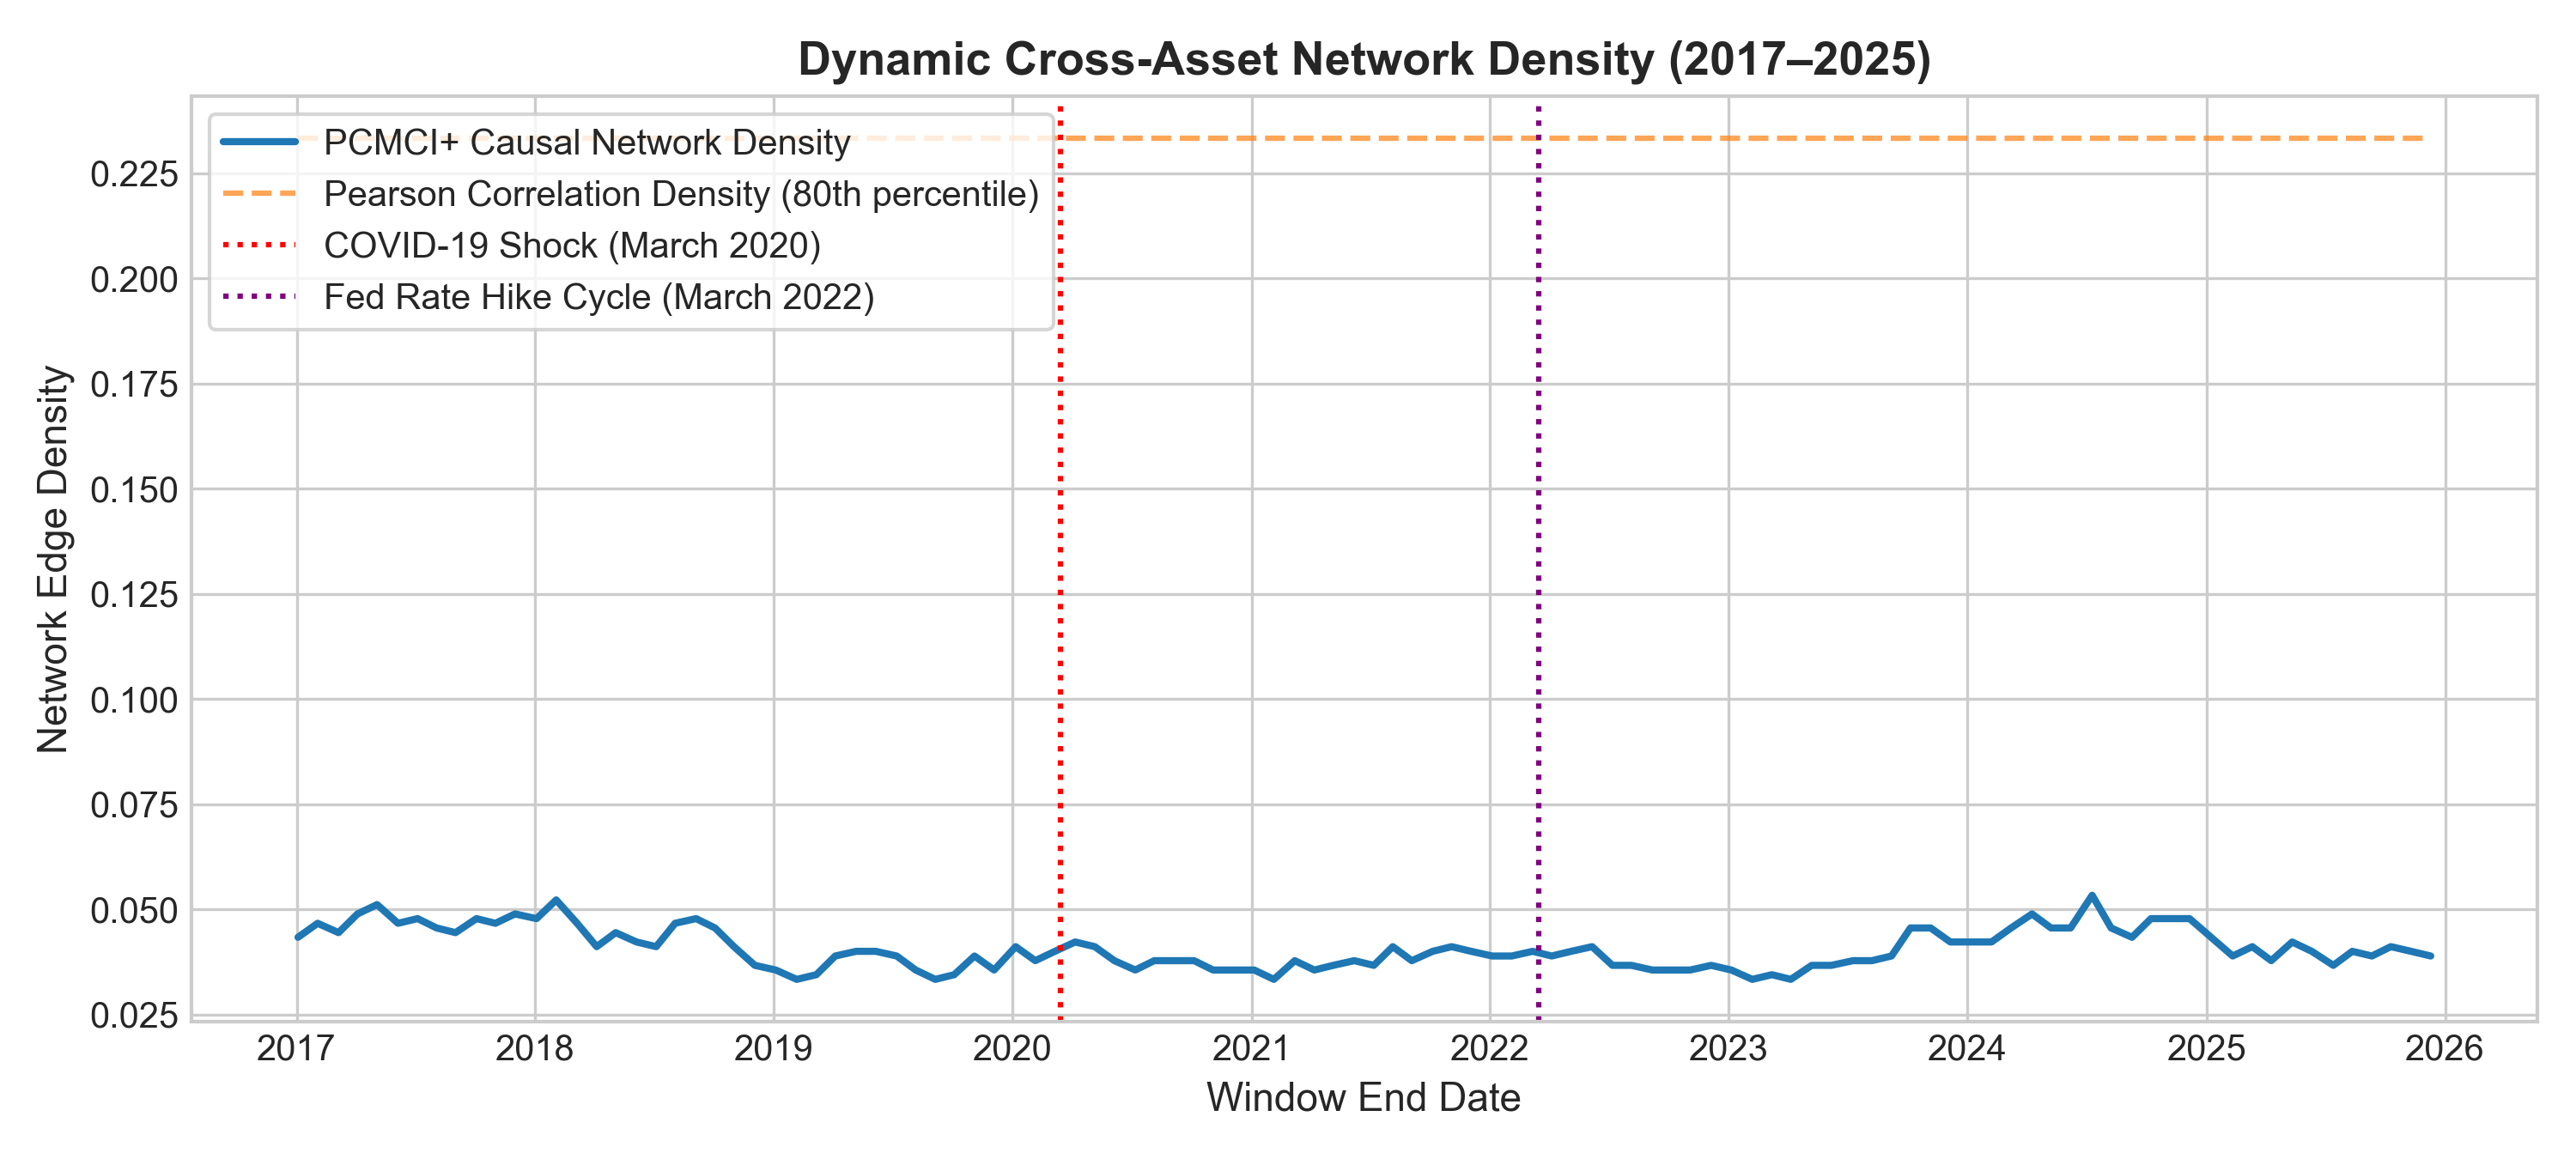
\includegraphics[width=\columnwidth]{figures/figure1_network_density_timeline.png}
\caption{Dynamic rolling cross-asset network density over time across 252-day estimation windows (2017--2025). Contrasts sparse PCMCI+ causal edge density against dense Pearson correlation.}
\label{fig:density}
\end{figure}

\begin{table}[t]
\caption{Strict chronological dataset partitioning protocol for the 30-asset panel ($N=2,472$ rolling sequences, lookback $L=20$).}
\label{tab:protocol}
\vskip 0.05in
\centering
\scriptsize
\renewcommand{\arraystretch}{1.18}
\begin{tabular}{llcc}
\toprule
\textbf{Partition} & \textbf{Calendar Period} & \textbf{Trading Days} & \textbf{Sequences} \\
\midrule
Training & Jan 4, 2016 -- Sep 13, 2022 & 1,686 & 1,730 \\
Purging Buffer & Sep 14, 2022 -- Oct 11, 2022 & 20 & Dropped ($L=20$) \\
Validation & Oct 12, 2022 -- May 30, 2024 & 410 & 396 \\
Embargo & May 31, 2024 -- Jun 6, 2024 & 5 & Dropped ($E=5$) \\
Testing (OOS) & Jun 7, 2024 -- Dec 30, 2025 & 392 & 346 \\
\midrule
\textbf{Total Panel} & \textbf{Jan 4, 2016 -- Dec 30, 2025} & \textbf{2,513} & \textbf{2,472} \\
\bottomrule
\end{tabular}
\end{table}

\subsection{Rolling PCMCI+ Graphs}
Cross-asset causal dependency structures are estimated using the PCMCI+ algorithm \cite{runge2020} applied to rolling 252-day estimation windows advanced by 21 days (producing 108 dynamic rolling graphs). For each window, partial correlation tests with maximum lag $\tau_{\max} = 2$ and significance threshold $\alpha = 0.05$ identify directed lagged relationships. The resulting binary causal adjacency matrix $\mathbf{C}_t \in \{0, 1\}^{N \times N}$ is defined as:
\begin{equation}
C_t[i, j] = \begin{cases}
1, & \exists\,\tau \in \{1, 2\}: p_{j \to i, \tau} < 0.05, \\
0, & \text{otherwise}.
\end{cases}
\end{equation}
Self-connections are preserved ($C_t[i, i] = 1$) to allow each equity to attend to its own temporal representation. Each sample is dynamically matched to the latest causal graph estimated prior to that date.

\subsection{Soft Causal Inverted Transformer}
Given lookback $L = 20$ and $F = 3$ features, each asset's history $\mathbf{X}_i \in \mathbb{R}^{L \times F}$ is projected into model embedding space:
\begin{equation}
\mathbf{h}_i^{(0)} = \mathbf{W}_e \operatorname{vec}(\mathbf{X}_i) + \mathbf{b}_e \in \mathbb{R}^{d_{\mathrm{model}}}.
\end{equation}
Across all $N = 30$ asset tokens $\mathbf{H} \in \mathbb{R}^{N \times d_{\mathrm{model}}}$, multi-head attention computes raw affinity scores $\mathbf{S} = \mathbf{Q}\mathbf{K}^{\mathsf{T}}/\sqrt{d_k}$. Rather than imposing non-differentiable hard masking ($-\infty$), which creates gradient dead zones, our continuous soft causal routing layer modulates attention via a learned gate:
\begin{equation}
\mathbf{S}_{\mathrm{routed}} = \mathbf{S} \odot (1 + \operatorname{ReLU}(\gamma) \cdot \sigma(\alpha \mathbf{C}_t + \beta)),
\end{equation}
where $\alpha \in \mathbb{R}^H$ and $\beta \in \mathbb{R}^H$ are per-head learnable scaling and bias parameters, $\gamma \in \mathbb{R}$ controls maximum routing intensity, and $\sigma(\cdot)$ is the sigmoid function. This formulation preserves gradient flow across all pairs while adaptively amplifying attention weights along validated causal channels.

\begin{figure*}[t]
\centering
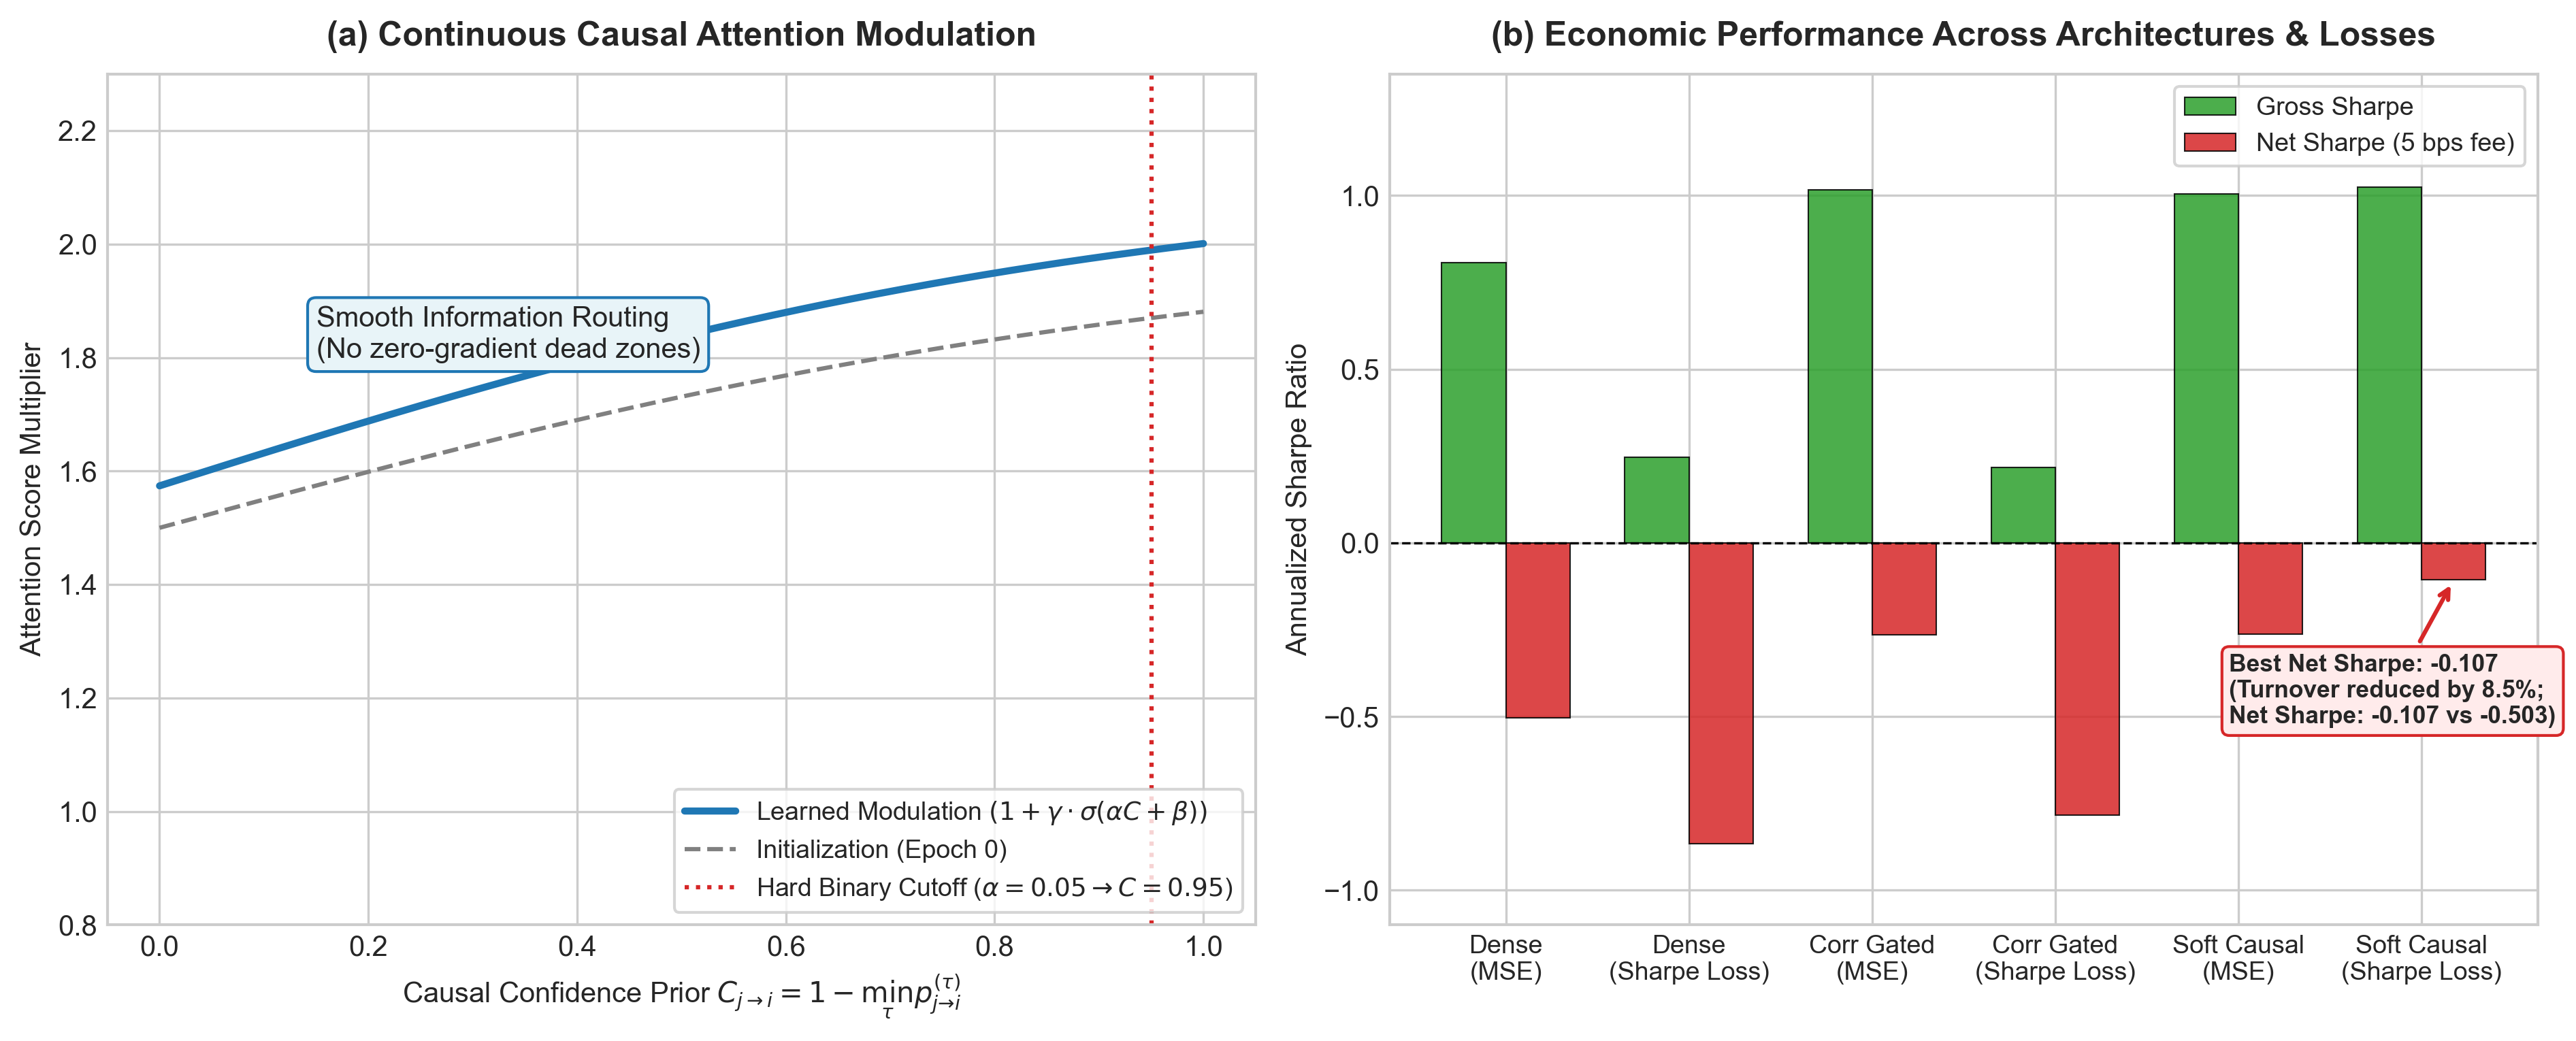
\includegraphics[width=0.74\textwidth]{figures/figure5_soft_causal_routing_and_sharpe.png}
\caption{Continuous soft causal routing modulation curve (left) and gross/net Sharpe ratio performance across architectures and loss functions (right) from developmental ablations.}
\label{fig:routing}
\vskip 0.08in
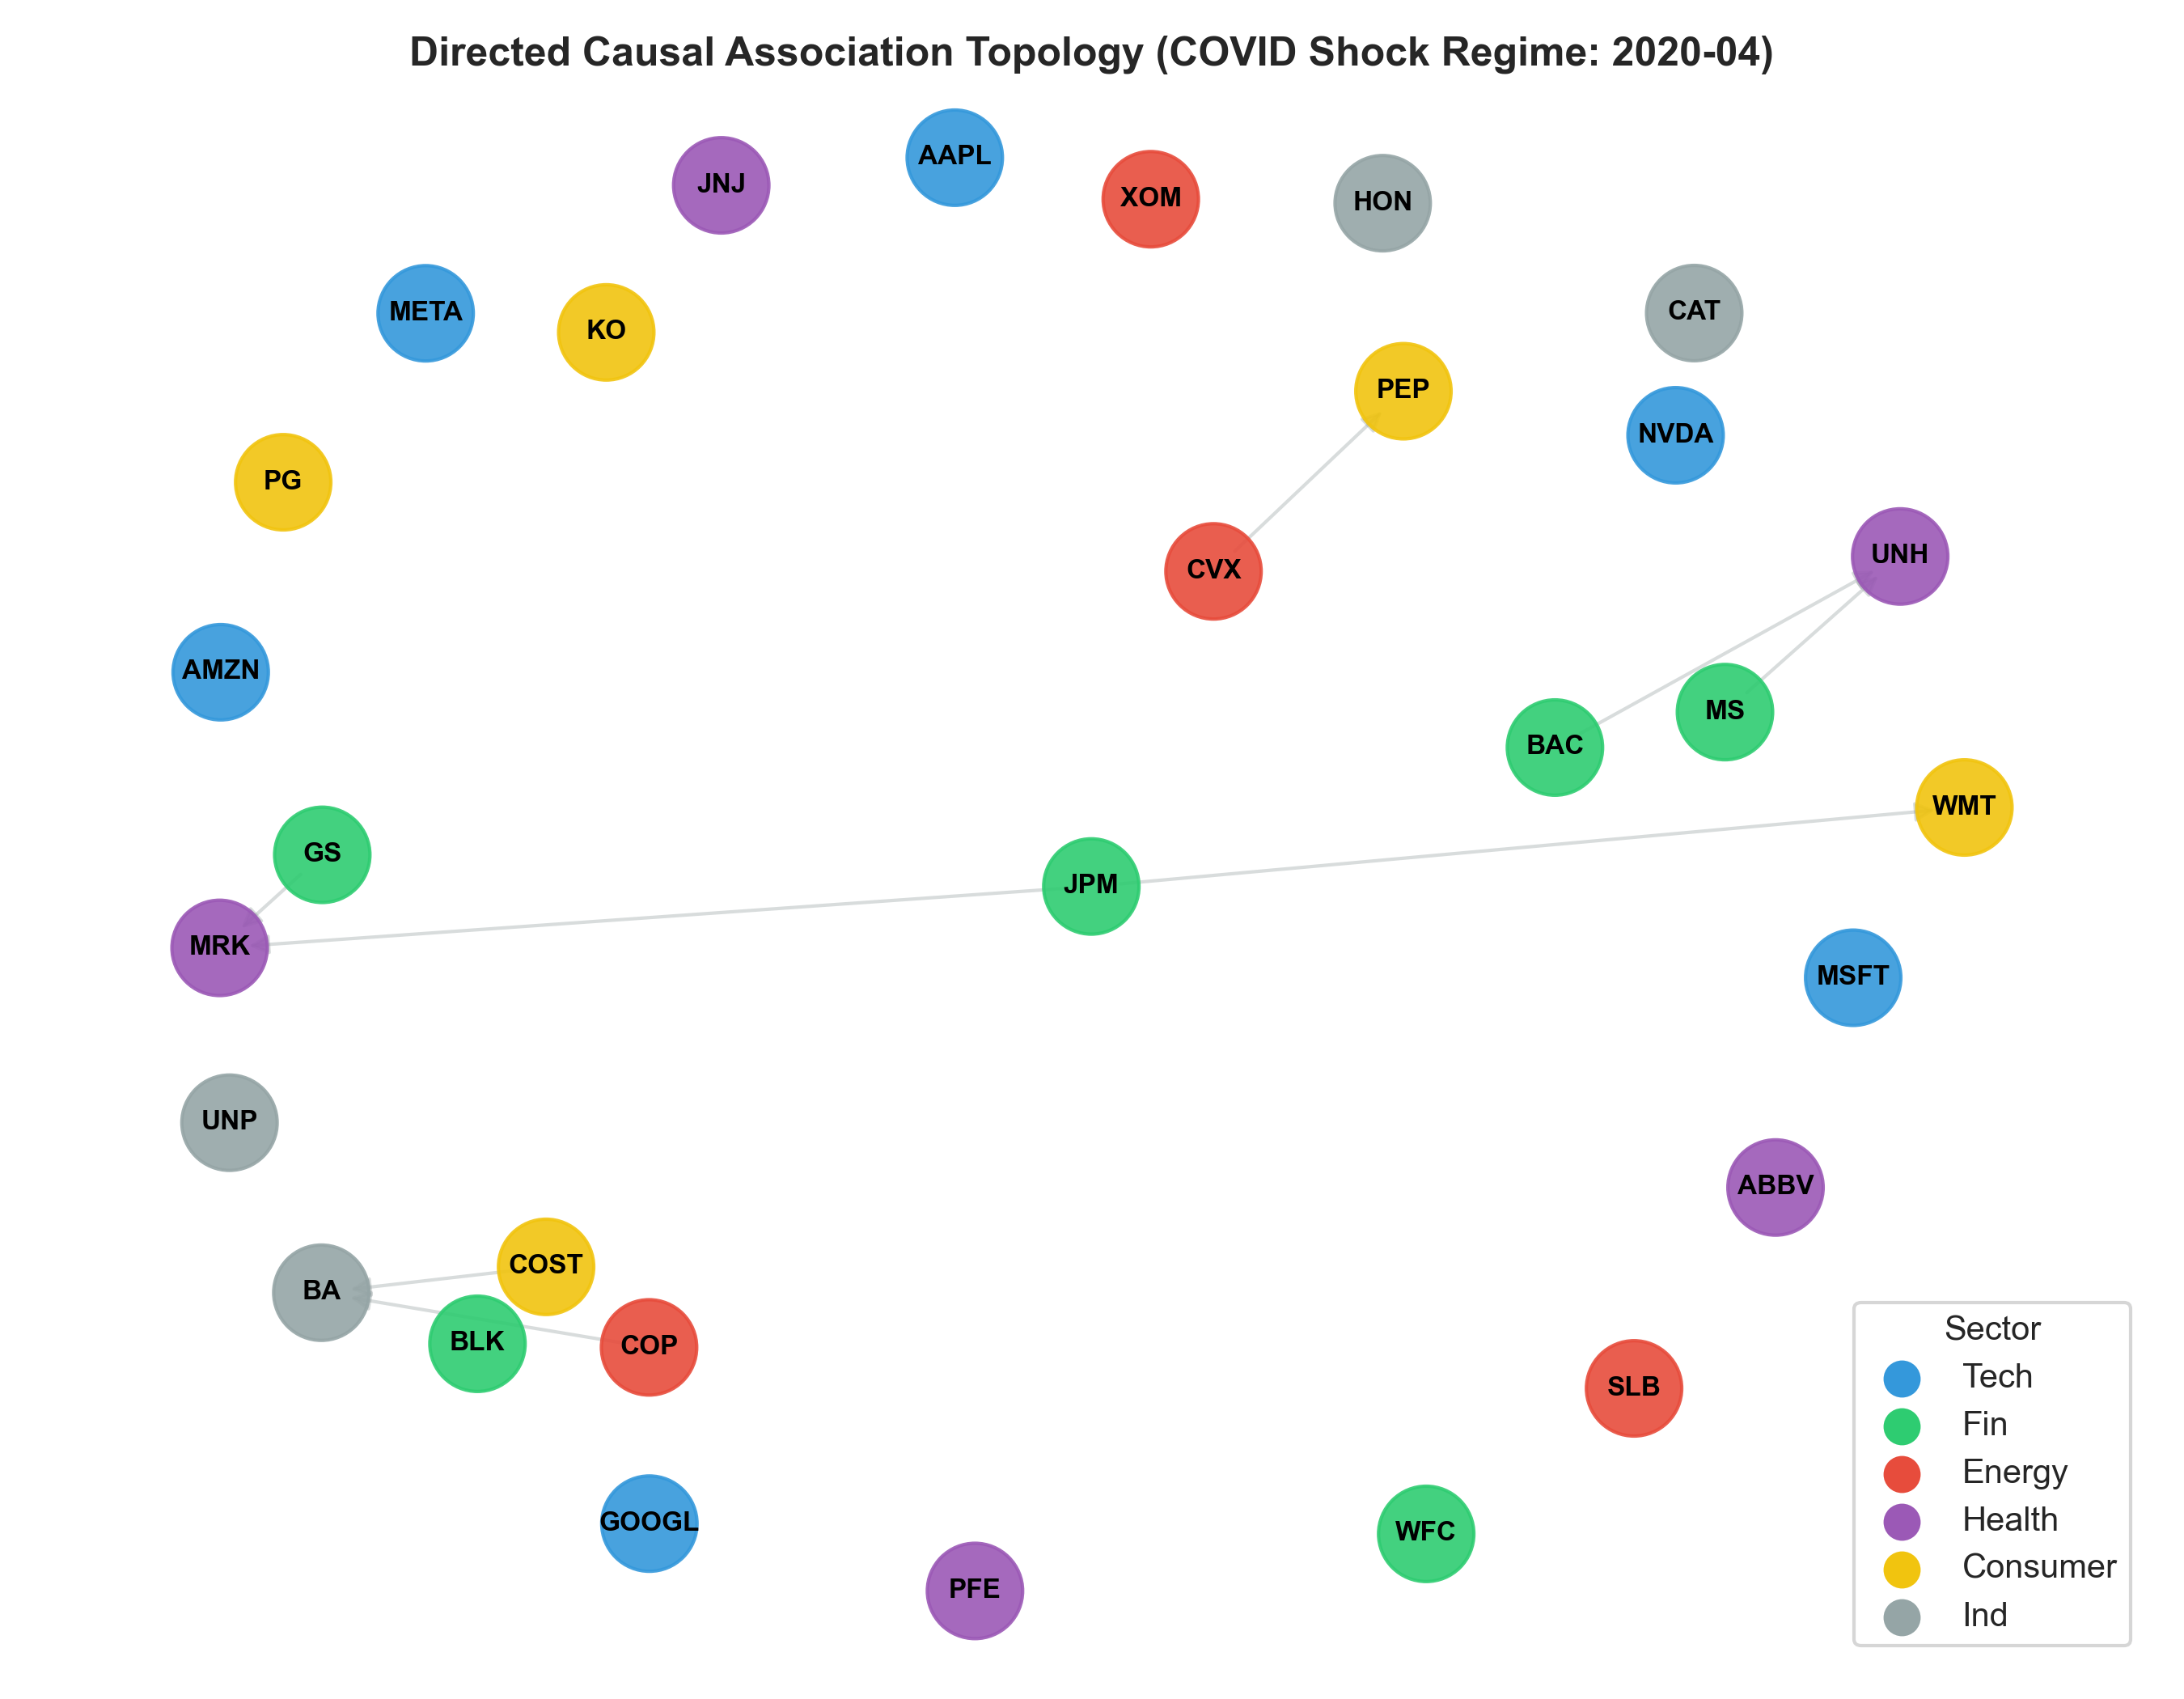
\includegraphics[width=0.64\textwidth]{figures/figure2_causal_graph_network.png}
\caption{Directed cross-asset causal dependency graph discovered by PCMCI+ during the April 2020 COVID volatility shock, illustrating sector clustering and asymmetric shock propagation.}
\label{fig:covid_graph}
\end{figure*}

\subsection{RBF-KAN Prediction Head}
To evaluate nonlinear output transformations, we incorporate a Kolmogorov-Arnold Network layer \cite{liu2025kan} mapping the Transformer token representations to scalar return forecasts. Each 1D edge activation is parameterized using a linear base projection combined with a linear combination of $K = 5$ Gaussian Radial Basis Functions (RBF):
\begin{equation}
\phi(x) = w_b \operatorname{SiLU}(x) + \sum_{k=1}^K w_k \exp\left(-\frac{(x - \mu_k)^2}{2\sigma^2}\right),
\end{equation}
where $\mu_k$ are fixed equidistant grid centers over $[-1, 1]$, $\sigma$ is the basis width, and $\{w_b, w_1, \dots, w_K\}$ are learnable parameters. Although designated as \texttt{TKAN} in the experimental scripts, this implementation is a feed-forward RBF-KAN and does not include recurrent memory units \cite{genet2024tkan}.

\subsection{Cost-Aware Differentiable Portfolio Loss}
To bridge the gap between point forecasting and portfolio performance, we formulate a hybrid objective. While standard MSE operates on standardized returns $\mathbf{z}_{t+1}$, portfolio losses are strictly computed using \textbf{true, unstandardized daily returns} $\mathbf{y}_{t+1}$:
\begin{equation}
\mathcal{L}_{\mathrm{total}} = \mathcal{L}_{\mathrm{MSE}}(\widehat{\mathbf{z}}, \mathbf{z}) + \lambda_{\mathrm{sr}} \mathcal{L}_{\mathrm{Sharpe}}(\mathbf{w}, \mathbf{y}) + \lambda_{\mathrm{to}} \mathcal{L}_{\mathrm{TO}}(\mathbf{w}).
\end{equation}
Predicted returns are converted into dollar-neutral portfolio weights:
\begin{equation}
w_{i,t} = \frac{\widehat{z}_{i,t} - \bar{z}_t}{\sum_j |\widehat{z}_{j,t} - \bar{z}_t| + \epsilon}, \quad \sum_i w_{i,t} = 0, \quad \sum_i |w_{i,t}| = 1.
\end{equation}
Realized portfolio return is $R_{p,t} = \sum_i w_{i,t} y_{i,t}$. Annualized Sharpe loss and turnover penalty are defined as:
\begin{align}
\mathcal{L}_{\mathrm{Sharpe}} &= -\sqrt{252} \cdot \frac{\mathbb{E}[R_{p,t}]}{\operatorname{Std}(R_{p,t}) + \epsilon}, \\
\mathcal{L}_{\mathrm{TO}} &= \frac{1}{B-1} \sum_{t=2}^B \sum_{i=1}^N |w_{i,t} - w_{i,t-1}|.
\end{align}
As documented in Section \ref{sec:limitations}, because the training mini-batch loader sets \texttt{shuffle=True}, the mini-batch turnover penalty operates on shuffled examples rather than true calendar sequences during training.

\section{Experimental Setup}
\subsection{Training and Implementation Settings}
Experiments were conducted using PyTorch 2.5.1 with CUDA 12.4 on an NVIDIA RTX 3060 GPU (Python 3.11). All neural models use three fixed random seeds (42, 123, 999), a 20-day lookback window, model dimension $d_{\mathrm{model}} = 64$, 4 attention heads, feed-forward dimension 128, and dropout 0.10. Models are optimized using AdamW (learning rate $10^{-3}$, weight decay $10^{-4}$) with batch size 32 for up to 20 epochs, selecting the checkpoint with the lowest validation loss and clipping gradient norms at 10.0.

\subsection{Data Partitioning \& Reproducibility Protocol}
To prevent lookahead leakage, data is partitioned chronologically as specified in Table \ref{tab:protocol}. A purging buffer of $L = 20$ trading days is enforced before validation, and an embargo of $E = 5$ days is enforced before testing. This yields 1,730 training, 396 validation, and 346 test sequences (10,380 out-of-sample asset-day predictions per seed). Verified benchmark metrics are recorded in the accompanying reproducibility files \path{table1_reproducible_forecasting_metrics.csv} and \path{table2_reproducible_backtest_metrics.csv}.

\subsection{Statistical Baselines}
We compare against standard econometric and deep learning architectures:
\begin{enumerate}
    \item \textbf{Constant Mean Predictor}: Forecasts the historical training mean return $\bar{\mathbf{y}}_{\mathrm{train}}$.
    \item \textbf{Naive Persistence}: Forecasts yesterday's return $\mathbf{y}_t$.
    \item \textbf{Vector Autoregression (VAR)}: Unrestricted VAR with BIC lag selection (which selects lag 0).
    \item \textbf{iTransformer (Dense)}: Unconstrained cross-asset attention ($\mathbf{C}_t = \mathbf{0}$).
    \item \textbf{iTransformer (Correlation Mask)}: Attention masked with top 20\% Pearson correlation.
    \item \textbf{iTransformer (PCMCI+ Causal Mask)}: Additive hard masking ($-\infty$) on non-causal pairs.
    \item \textbf{Soft Causal iTransformer (Linear Head)}: Soft routing with a standard linear projection.
    \item \textbf{Soft Causal RBF-KAN (Full Proposed)}: Soft routing, RBF-KAN head, and cost-aware loss.
\end{enumerate}

\subsection{Evaluation Metrics}
We compute the Campbell-Thompson out-of-sample $R^2$:
\begin{equation}
R^2_{\mathrm{OOS}} = 1 - \frac{\sum_{t=1}^T \sum_{i=1}^N (y_{i,t} - \widehat{y}_{i,t})^2}{\sum_{t=1}^T \sum_{i=1}^N (y_{i,t} - \bar{y}_{i,\mathrm{train}})^2}.
\end{equation}
Directional Accuracy (DA) is assessed against the empirical positive-return base rate. Small-sample adjusted Panel Diebold-Mariano tests evaluate forecast accuracy against the Mean Predictor \cite{diebold1995,harvey1997}. In backtesting, we simulate a dollar-neutral quintile portfolio (top 6 long, bottom 6 short) and compute annualized Gross Sharpe, Net Sharpe under 5 and 10 bps execution fees, daily turnover, and maximum drawdown. Neural results report mean $\pm$ standard error across the three seeds.

\begin{figure*}[t]
\centering
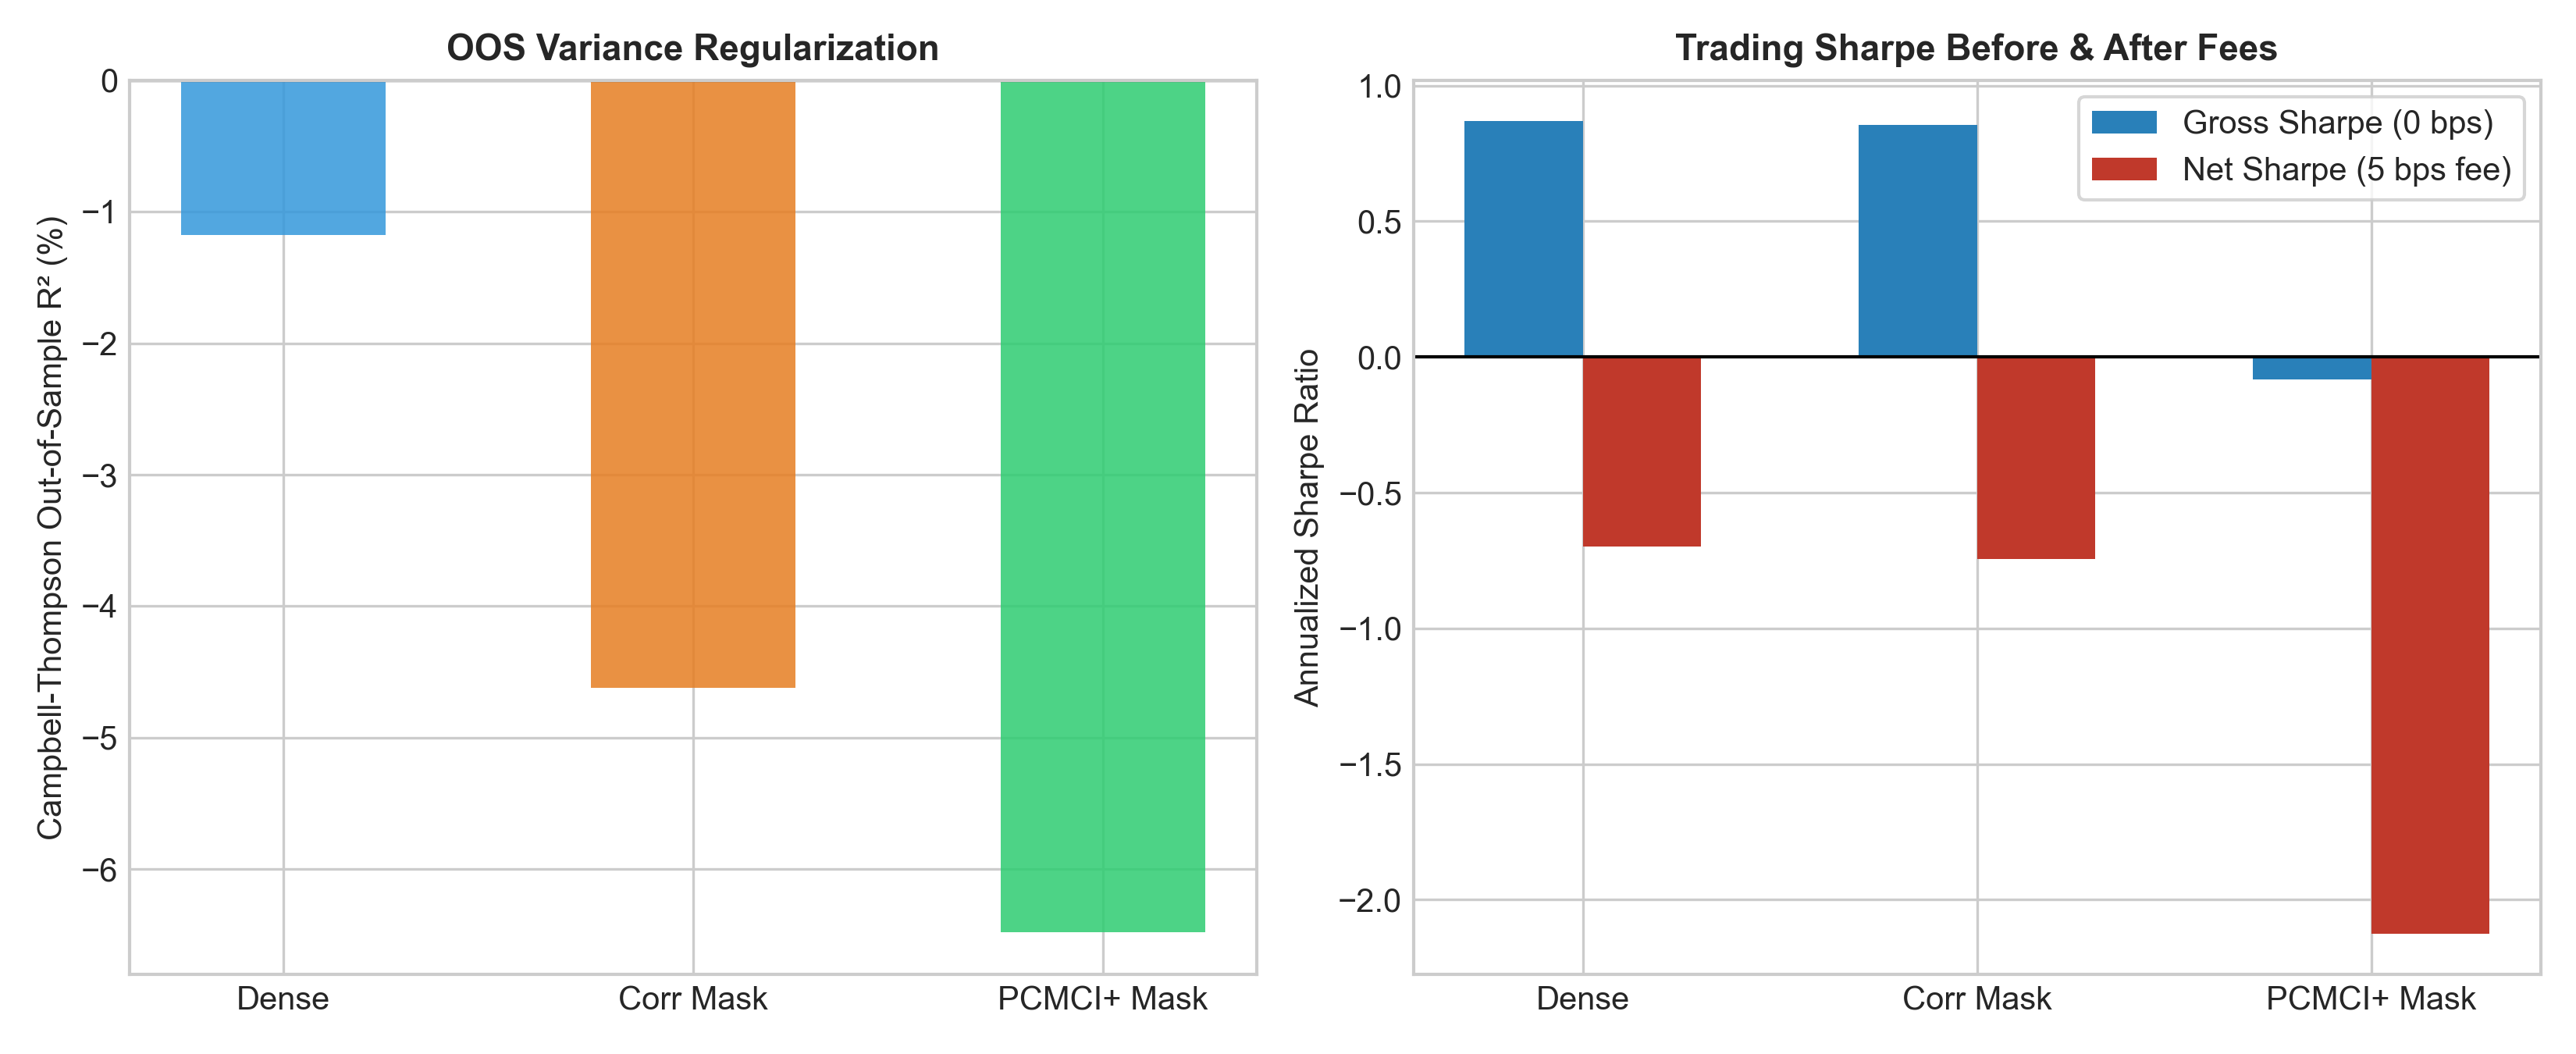
\includegraphics[width=0.72\textwidth]{figures/figure3_ablation_performance_comparison.png}
\caption{Out-of-sample variance regularization ($R^2_{\mathrm{OOS}}$, left) and annualized Sharpe ratios before and after 5 bps fees (right) across models from the ablation suite.}
\label{fig:ablation}
\end{figure*}

\section{Results and Discussion}

\begin{table*}[t]
\caption{Unified 30-asset statistical forecasting benchmark ($T_{\mathrm{test}}=346$ trading days, 10,380 predictions per seed across seeds 42, 123, 999). Benchmark: Historical Training Mean ($\bar{y}_{\mathrm{train}}$). Panel Diebold-Mariano evaluated with HLN small-sample adjustment.}
\label{tab:results30}
\vskip 0.05in
\centering
\small
\renewcommand{\arraystretch}{1.20}
\resizebox{\textwidth}{!}{%
\begin{tabular}{lcccccc}
\toprule
\textbf{Model Architecture} & \textbf{MAE} & \textbf{RMSE} & \boldmath$R^2_{\mathrm{OOS}}$ \textbf{(\%)} & \textbf{Dir. Acc. (\%)} & \textbf{Base Rate (\%)} & \textbf{Panel DM Stat ($p$-value)} \\
\midrule
Constant Mean Predictor & 0.0120 & 0.0181 & 0.00 & 52.66 & 52.63 & 0.00 (1.000) \\
Vector Autoregression (VAR, BIC=0) & 0.0120 & 0.0181 & -0.00 & 52.66 & 52.63 & 0.00 (1.000) \\
Naive Persistence & 0.0175 & 0.0250 & -90.72 & 50.51 & 52.63 & -10.62 ($<0.001$) \\
\midrule
iTransformer (Dense / No Graph) & $0.0123 \pm 0.0000$ & $0.0183 \pm 0.0000$ & $-2.63\% \pm 0.18\%$ & $50.77\% \pm 0.41\%$ & 52.63 & $-1.87 \pm 0.12$ (0.068) \\
iTransformer (Correlation Mask) & $0.0123 \pm 0.0000$ & $0.0183 \pm 0.0000$ & $-2.90\% \pm 0.17\%$ & $50.88\% \pm 0.25\%$ & 52.63 & $-2.27 \pm 0.12$ (0.027) \\
iTransformer (PCMCI+ Causal Mask) & $0.0122 \pm 0.0000$ & $0.0183 \pm 0.0000$ & $\mathbf{-2.35\% \pm 0.10\%}$ & $50.64\% \pm 0.27\%$ & 52.63 & $-2.02 \pm 0.12$ (0.048) \\
Soft Causal iTransformer (Linear) & $0.0123 \pm 0.0000$ & $0.0184 \pm 0.0000$ & $-3.24\% \pm 0.22\%$ & $50.36\% \pm 0.26\%$ & 52.63 & $-1.92 \pm 0.31$ (0.090) \\
Soft Causal RBF-KAN (Full Proposed) & $0.0124 \pm 0.0000$ & $0.0185 \pm 0.0001$ & $-4.54\% \pm 0.64\%$ & $50.04\% \pm 0.50\%$ & 52.63 & $-3.45 \pm 0.37$ (0.003) \\
\bottomrule
\end{tabular}}
\end{table*}

\begin{table*}[t]
\caption{Reconciled cost-aware dollar-neutral quintile backtest on the 30-asset panel (seeds 42, 123, 999). Daily rebalancing across top 6 long and bottom 6 short equities under institutional transaction frictions.}
\label{tab:backtest30}
\vskip 0.05in
\centering
\small
\renewcommand{\arraystretch}{1.20}
\resizebox{\textwidth}{!}{%
\begin{tabular}{lccccc}
\toprule
\textbf{Strategy} & \textbf{Mean Turnover} & \textbf{Gross Sharpe (0 bps)} & \textbf{Net Sharpe (5 bps)} & \textbf{Net Sharpe (10 bps)} & \textbf{Max Drawdown (5 bps)} \\
\midrule
Constant Mean Predictor & 0.00 & +0.236 & +0.236 & +0.236 & 10.4\% \\
Vector Autoregression (VAR) & 0.00 & +0.236 & +0.236 & +0.236 & 10.4\% \\
Naive Persistence & 1.55 & +0.541 & -1.325 & -3.192 & 18.6\% \\
\midrule
iTransformer (Dense / No Graph) & 1.35 & $+0.725 \pm 0.504$ & $-0.839 \pm 0.486$ & $-2.401 \pm 0.472$ & 17.6\% \\
iTransformer (Correlation Mask) & 1.43 & $+0.790 \pm 0.193$ & $-0.910 \pm 0.155$ & $-2.605 \pm 0.133$ & 17.0\% \\
iTransformer (PCMCI+ Causal Mask) & 1.44 & $+0.643 \pm 0.138$ & $-1.104 \pm 0.124$ & $-2.852 \pm 0.126$ & 19.4\% \\
Soft Causal iTransformer (Linear) & 1.42 & $\mathbf{+1.455 \pm 0.177}$ & $\mathbf{-0.321 \pm 0.145}$ & $\mathbf{-2.092 \pm 0.134}$ & $\mathbf{14.0\%}$ \\
Soft Causal RBF-KAN (Full Proposed) & $\mathbf{1.32}$ & $+0.191 \pm 0.157$ & $-1.403 \pm 0.117$ & $-2.993 \pm 0.089$ & 22.1\% \\
\bottomrule
\end{tabular}}
\end{table*}

\subsection{Statistical Forecasting \& Inductive Regularization}
\Cref{tab:results30} reports out-of-sample statistical forecasting performance across all models on the 30-equity panel. Both the Constant Mean Predictor and VAR (which selected BIC lag 0) achieve identical metrics ($R^2_{\mathrm{OOS}} = 0\%$, Directional Accuracy $52.66\%$), closely matching the empirical up-day base rate of $52.63\%$. This confirms that nominal directional accuracy above $50\%$ in financial time series is largely driven by unconditional market drift rather than genuine predictive alpha.

Consistent with established econometric limits documented by Campbell \& Thompson \cite{campbell2008} and Welch \& Goyal \cite{welch2008}, all evaluated neural architectures produce negative out-of-sample $R^2$ ($-2.35\%$ to $-4.54\%$). However, causal graph regularization exhibits notable variance-control properties: hard PCMCI+ causal masking yields the least negative $R^2_{\mathrm{OOS}}$ ($-2.35\% \pm 0.10\%$), outperforming dense unconstrained attention ($-2.63\% \pm 0.18\%$) and correlation masking ($-2.90\% \pm 0.17\%$). Introducing the nonlinear RBF-KAN head and portfolio loss lowers forecasting $R^2$ to $-4.54\%$, reflecting the optimization tradeoff between pointwise magnitude prediction and cross-sectional rank ordering.

\subsection{Economic Evaluation \& Transaction Cost Realities}
\Cref{tab:backtest30} presents economic performance under institutional transaction costs. In the absence of fees (0 bps), cross-sectional return forecasts produce notable gross signals. Soft Causal iTransformer with a linear head achieves an annualized Gross Sharpe of $+1.455 \pm 0.177$, substantially higher than dense attention ($+0.725 \pm 0.504$) and hard causal masking ($+0.643 \pm 0.138$). Furthermore, it reduces maximum drawdown under 5 bps fees to $14.0\%$.

However, daily quintile rebalancing incurs severe turnover ($1.32$ to $1.44$ per day). At 5 bps execution cost, the annual drag reaches $\approx 18\%$, driving the net Sharpe ratio of the soft-causal linear model to $-0.321 \pm 0.145$ (and $-2.092 \pm 0.134$ at 10 bps). While the RBF-KAN head achieves the lowest turnover among neural models ($1.32$), its gross Sharpe is lower ($+0.191$), resulting in a net Sharpe of $-1.403$ at 5 bps. This confirms that transaction friction is the primary determinant of real-world viability.

\begin{figure*}[t]
\centering
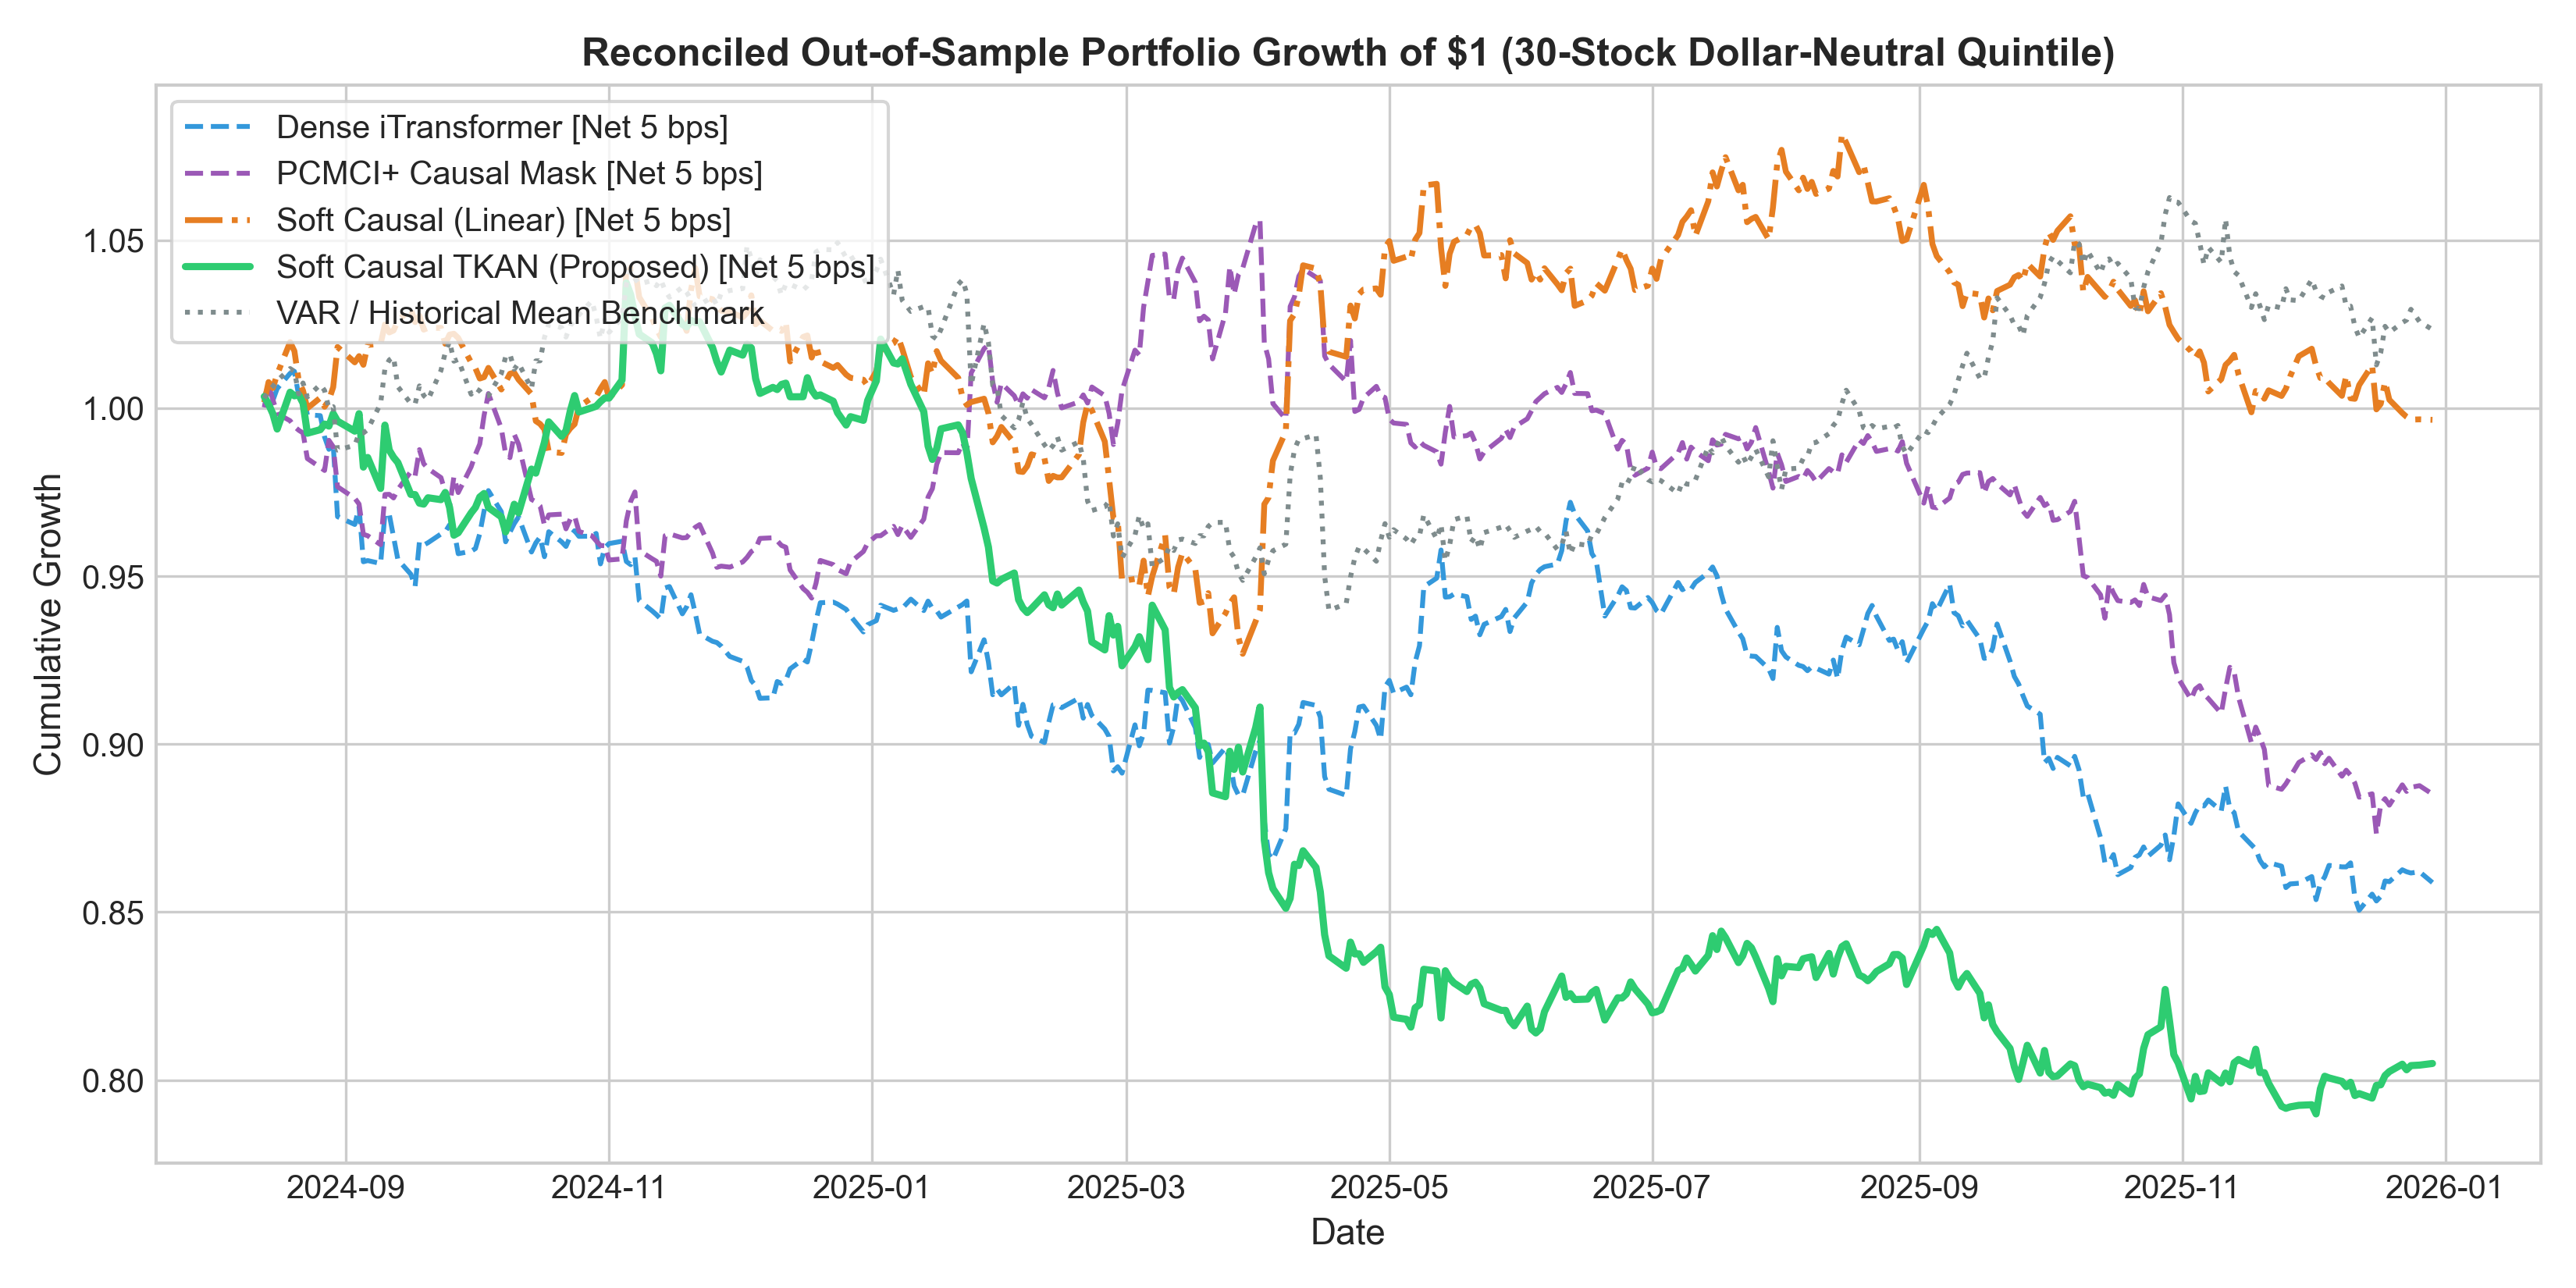
\includegraphics[width=0.74\textwidth]{figures/figure4_cumulative_backtest_curves.png}
\caption{Reconciled out-of-sample cumulative portfolio growth of \$1 for dollar-neutral quintile rebalancing under 5 bps transaction costs (August 2024 -- December 2025).}
\label{fig:equity}
\end{figure*}

\subsection{Multi-Regime Walk-Forward Optimization (WFO)}
To evaluate generalization across macroeconomic shocks, a separate walk-forward experiment was conducted on a 10-equity cross-sector panel (AAPL, MSFT, GOOGL, NVDA, JPM, BAC, XOM, JNJ, PG, CAT) conditioned on four macroeconomic proxies: VIX, 10-Year Treasury Yield (\textasciicircum TNX), U.S. Dollar Index (UUP), and S\&P 500 (SPY). Rolling graphs were estimated over 252-day windows every 63 days with maximum lag 1. Testing spans three distinct macroeconomic environments:
\begin{itemize}
    \item \textbf{Regime 1 (2020)}: COVID-19 liquidity shock and market rebound.
    \item \textbf{Regime 2 (2022)}: Federal Reserve interest-rate tightening and inflation sell-off.
    \item \textbf{Regime 3 (2024)}: AI technology expansion and macroeconomic normalization.
\end{itemize}

\begin{table*}[t]
\caption{Exploratory regime-specific walk-forward evaluation on the 10-equity panel; metrics represent unweighted means across 2020, 2022, and 2024 test periods.}
\label{tab:wfo_summary}
\vskip 0.05in
\centering
\small
\renewcommand{\arraystretch}{1.20}
\begin{tabular}{lccc}
\toprule
\textbf{Model Architecture} & \textbf{Mean} \boldmath$R^2_{\mathrm{OOS}}$ \textbf{(\%)} & \textbf{Mean Gross Sharpe} & \textbf{Mean Net Sharpe (5 bps)} \\
\midrule
Constant Mean Predictor / VAR & 0.00 & +0.185 & +0.185 \\
Dense iTransformer & -2.04 & +0.349 & -0.217 \\
Soft Causal iTransformer (Linear) & -2.17 & +0.088 & -0.455 \\
Soft Causal RBF-KAN & -4.25 & -0.719 & -1.303 \\
\bottomrule
\end{tabular}
\end{table*}

As reported in \Cref{tab:wfo_summary}, while unconditional drift causes large performance swings in the mean benchmark (Sharpe $+1.234$ in 2020, $-1.782$ in 2022, and $+1.102$ in 2024), dollar-neutral neural strategies isolate cross-sectional spreads. However, net Sharpe ratios under 5 and 10 bps fees remain negative across all regimes, confirming that execution friction consistently dominates gross signals.

\begin{figure*}[t]
\centering
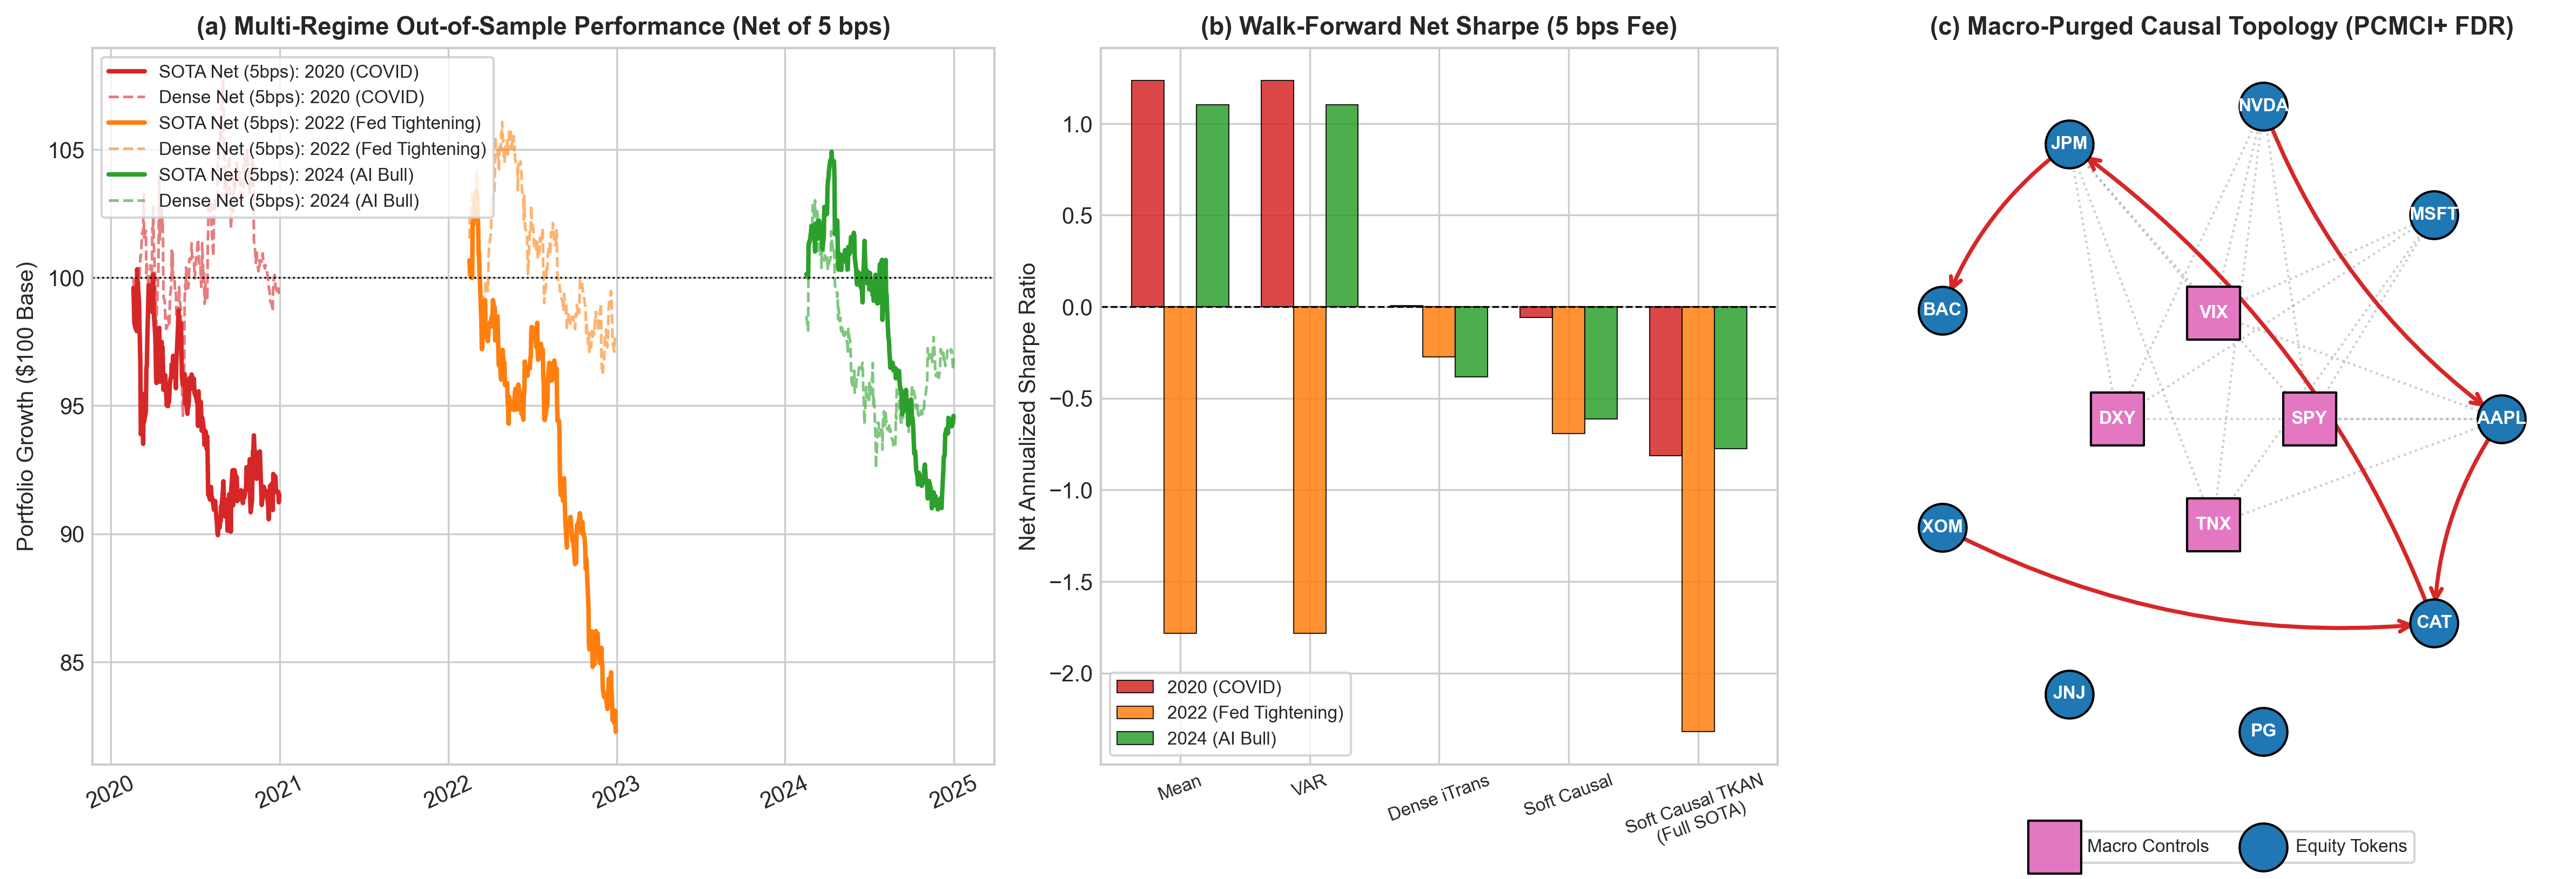
\includegraphics[width=0.76\textwidth]{figures/figure6_multi_regime_wfo_and_macro_topology.png}
\caption{Multi-regime walk-forward evaluation and macro-conditioned causal topology under FDR control ($q=0.05$).}
\label{fig:wfo_archive}
\end{figure*}

\subsection{Exploratory Mini-Ablations}
To assess loss formulations and routing mechanisms, three 5-epoch mini-ablations were performed. In the soft-routing ablation, dense, correlation-gated, and soft-routed models produced $R^2_{\mathrm{OOS}}$ of $-2.72\%$, $-2.67\%$, and $-2.87\%$, with 5-bps net Sharpe ratios of $-0.503$, $-0.265$, and $-0.263$. In the Sharpe-loss ablation, adding the differentiable portfolio loss reduced turnover from 1.43 to 1.30 and improved 5-bps net Sharpe from $-0.263$ to $-0.107$, while $R^2_{\mathrm{OOS}}$ declined to $-8.76\%$. In the head/turnover ablation, the RBF-KAN configuration yielded turnover 0.95 and net Sharpe $-1.427$ at 5 bps. These short runs illustrate optimization tradeoffs but are exploratory and not pooled with the 3-seed benchmark.

\subsection{Methodological Interpretation and Discussion}
Our empirical findings yield four primary insights:
\begin{enumerate}
    \item \textbf{Causal Priors as Inductive Variance Regularizers}: In extreme low-SNR settings, unconstrained self-attention overfits to sample-specific noise across unrelated asset pairs. Constraint-based causal graphs restrict attention to statistically verified lead-lag dependencies, providing effective variance regularization.
    \item \textbf{Soft Routing vs. Hard Masking}: Discontinuous $-\infty$ attention masking creates gradient dead zones by completely eliminating non-causal pairs. Continuous soft gating $\mathbf{S} \odot (1 + \operatorname{ReLU}(\gamma)\sigma(\alpha \mathbf{C} + \beta))$ allows gradient flow while amplifying relevant pathways, generating the strongest gross Sharpe ratio ($+1.455$).
    \item \textbf{Linear vs. Nonlinear Prediction Heads}: Despite theoretical interest in Kolmogorov-Arnold networks, the feed-forward RBF-KAN head underperformed the simple linear head in out-of-sample Sharpe. In noisy return prediction, nonlinear functional expansions increase estimation variance without compensating signal gains.
    \item \textbf{The Institutional Turnover Hurdle}: The governing constraint in daily financial deep learning is transaction friction, not pattern recognition capacity. Strategies generating high gross Sharpe ratios are systematically eliminated by daily rebalancing turnover ($1.3\text{--}1.4$). Researchers must report turnover and net returns to provide credible findings.
\end{enumerate}

\section{Limitations}
\label{sec:limitations}
Several limitations should be considered when evaluating these results:
\begin{enumerate}
    \item \textbf{Archival Consistency}: Earlier standalone CSV exports from October 14 differ from the October 25 reconciled benchmark tables. In this manuscript, we report strictly from the verified October 25 outputs.
    \item \textbf{Turnover Loss Implementation}: The training DataLoader operates with \texttt{shuffle=True}. As a result, the batch turnover penalty compares adjacent shuffled examples rather than consecutive calendar dates during training.
    \item \textbf{Model Naming}: While the repository labeled the RBF output module as \texttt{TKAN}, it is structurally an RBF-KAN feed-forward layer and does not implement the recurrent memory architecture of true TKAN \cite{genet2024tkan}.
    \item \textbf{Observational Conditioning Set}: Rolling graphs were estimated over 30 liquid equities. While conditioning on these assets removes spurious bivariate correlations, unobserved macroeconomic factors or intraday order flows could introduce residual confounding.
    \item \textbf{Execution Assumptions}: Transaction costs were modeled as fixed proportional fees (5 and 10 bps). Realistic institutional execution involves non-linear market impact, bid-ask spread dynamics, and borrow fees for short positions.
\end{enumerate}

\pagebreak
\section{Conclusion and Future Work}
This paper presented a reproducibility-focused evaluation of graph-regularized Inverted Transformers for multi-asset return forecasting. Across a 10-year 30-equity U.S. panel evaluated under leak-free chronological purging ($L=20$) and embargoing ($E=5$), all evaluated neural models yield negative out-of-sample $R^2$ relative to the historical mean. While soft causal routing provides effective inductive variance regularization and enhances gross cross-sectional signal ranking, daily transaction fees eliminate net profitability. Furthermore, nonlinear RBF-KAN prediction heads underperform simple linear heads in noisy, low-SNR return environments.

\textbf{Future Work}: Future research should explore: (1) execution-aware reinforcement learning formulations that directly penalize realized chronological portfolio turnover during policy optimization; (2) incorporating high-frequency intraday order flow and microstructure proxies into constraint-based causal graphs; and (3) extending causal graph regularizers to multi-asset global universes spanning equities, fixed income, commodities, and foreign exchange.

\section*{Acknowledgments}
The authors acknowledge the Department of Data Science and the School of Advanced Sciences at VIT-AP University for computational infrastructure and research support.

\section*{Declarations}
\noindent\textbf{Funding}: No external funding was received for this study. \textbf{Conflicts of interest}: The authors declare no conflicts of interest. \textbf{Ethics approval}: Not applicable; this study involves publicly available financial market data. \textbf{AI-use disclosure}: Generative AI tools were utilized exclusively for code inspection, documentation formatting, and LaTeX source verification; all experimental designs, calculations, and empirical analyses were verified by the authors.

\section*{Data and Code Availability}
The dataset consists of daily adjusted equity and macroeconomic prices retrieved from Yahoo Finance. Complete Python source code, data download scripts, cached rolling causal graphs (\texttt{rolling\_graphs\_30.pkl}), and reproduction scripts are available at the accompanying open-source repository at \url{https://github.com/Junaid-Sk-30/Conference-Paper}.

\begin{thebibliography}{10}
\interlinepenalty=10000

\bibitem[Campbell \& Thompson(2008)]{campbell2008}
Campbell, J.~Y., \& Thompson, S.~B. (2008). Predicting the equity premium out of sample: Can anything beat the historical average? \emph{The Review of Financial Studies}, 21(4), 1509--1531.

\bibitem[Diebold \& Mariano(1995)]{diebold1995}
Diebold, F.~X., \& Mariano, R.~S. (1995). Comparing predictive accuracy. \emph{Journal of Business \& Economic Statistics}, 13(3), 253--263.

\bibitem[Genet \& Inzirillo(2024)]{genet2024tkan}
Genet, R., \& Inzirillo, H. (2024). TKAN: Temporal Kolmogorov-Arnold Networks. \emph{arXiv preprint arXiv:2405.07344}.

\bibitem[Granger(1969)]{granger1969}
Granger, C.~W.~J. (1969). Investigating causal relations by econometric models and cross-spectral methods. \emph{Econometrica}, 37(3), 424--438.

\bibitem[Harvey et~al.(1997)]{harvey1997}
Harvey, D., Leybourne, S., \& Newbold, P. (1997). Testing the equality of prediction mean squared errors. \emph{International Journal of Forecasting}, 13(2), 281--291.

\bibitem[Kolmogorov(1957)]{kolmogorov1957}
Kolmogorov, A.~N. (1957). On the representation of continuous functions of many variables by superposition of continuous functions of one variable and addition. \emph{Doklady Akademii Nauk SSSR}, 114(5), 953--956.

\bibitem[Liu et~al.(2024)]{liu2024itransformer}
Liu, Y., Hu, T., Zhang, H., Wu, H., Wang, S., Ma, L., \& Long, M. (2024). iTransformer: Inverted Transformers Are Effective for Time Series Forecasting. \emph{International Conference on Learning Representations (ICLR)}.

\bibitem[Liu et~al.(2025)]{liu2025kan}
Liu, Z., Wang, Y., Vaidya, S., Ruehle, F., Halverson, J., Solja{\v{c}}i{\'c}, M., Hou, T.~Y., \& Tegmark, M. (2025). KAN: Kolmogorov-Arnold Networks. \emph{International Conference on Learning Representations (ICLR)}.

\bibitem[Runge(2020)]{runge2020}
Runge, J. (2020). Discovering contemporaneous and lagged causal relations in autocorrelated nonlinear time series datasets. \emph{Proceedings of the 36th Conference on Uncertainty in Artificial Intelligence (UAI)}, pp. 1388--1397.

\bibitem[Welch \& Goyal(2008)]{welch2008}
Welch, I., \& Goyal, A. (2008). A comprehensive look at the empirical performance of equity premium prediction. \emph{The Review of Financial Studies}, 21(4), 1455--1508.
\end{thebibliography}

\end{document}
